\section{Observation and Calculations}

\noindent Least Count of oscilloscope $=0.2$ V, $P = 5$ V

\begin{table}[H]
    \centering
        \caption{Table for measurement of $g$ at $\nu= 13.03$ MHz}
        \begin{tabular}{|c|c|c|c|c|} \hline
        Current (I) & 2Q & Q & Magnetic Field & $H_{pp}$ \\ 
        (mA) & (V) & (V) & H (mT) & (Gauss)\\ \hline
        99 & 3.2 & 1.60  & 0.51 & 14.42 \\
        126 & 2.4 & 1.20  & 0.72 & 20.36 \\
        153 & 1.8 & 0.90  & 0.86 & 24.32 \\
        180 & 1.6 & 0.80  & 0.99 & 28.00   \\
        207 & 1.4 & 0.70  & 1.14 & 32.24 \\
        230 & 1.2 & 0.60  & 1.27 & 35.92 \\
        257 & 1.1 & 0.55 & 1.44 & 40.73 \\
        282 & 1.0 & 0.50  & 1.51 & 42.71 \\
        307 & 0.9 & 0.45 & 1.63 & 46.10 \\ \hline
    \end{tabular}    
    \label{tab:1}
\end{table}

\begin{figure}[H]
    \centering
    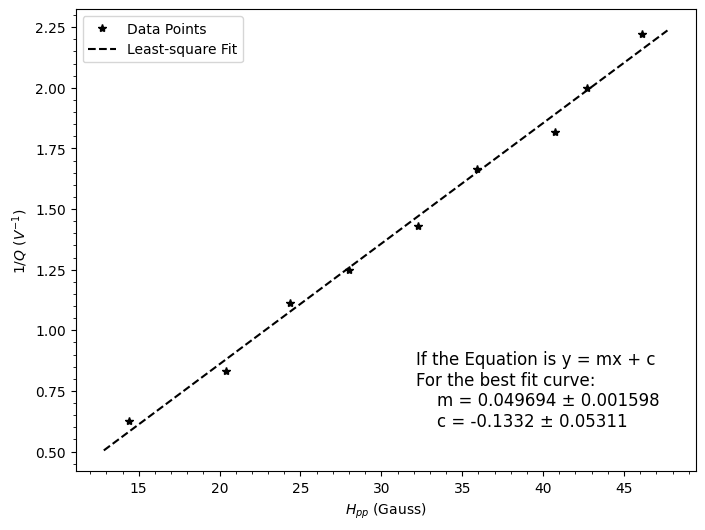
\includegraphics[width=1\columnwidth]{images/1.png}
    \caption{Plot of 1/Q vs. $H_{pp}$ at $\nu= 13.03$ MHz}
    \label{g1}
\end{figure}

From Fig. \ref{g1}, slope $= 0.0497$. Putting $P=5$ V, we get $H_0=4.02$ Gauss and hence, $g=2.31$.

\begin{table}[H]
    \centering
        \caption{Table for measurement of $g$ at $\nu= 14.01$ MHz}
        \begin{tabular}{|c|c|c|c|c|} \hline
        Current (I) & 2Q & Q & Magnetic Field & $H_{pp}$ \\ 
        (mA) & (V) & (V) & H (mT) & (Gauss)\\ \hline
        99 & 3.4 & 1.70  & 0.51 & 14.42 \\
        127 & 2.6 & 1.30  & 0.72 & 20.36 \\
        154 & 2.0   & 1.00    & 0.86 & 24.32 \\
        184 & 1.7 & 0.85 & 0.99 & 28.00    \\
        209 & 1.5 & 0.75 & 1.14 & 32.24 \\
        233 & 1.3 & 0.65 & 1.27 & 35.92 \\
        258 & 1.1 & 0.55 & 1.44 & 40.73 \\
        282 & 1.0   & 0.50  & 1.51 & 42.71 \\
        307 & 0.9 & 0.45 & 1.63 & 46.10  \\ \hline
    \end{tabular}    
    \label{tab:2}
\end{table}

\begin{figure}[H]
    \centering
    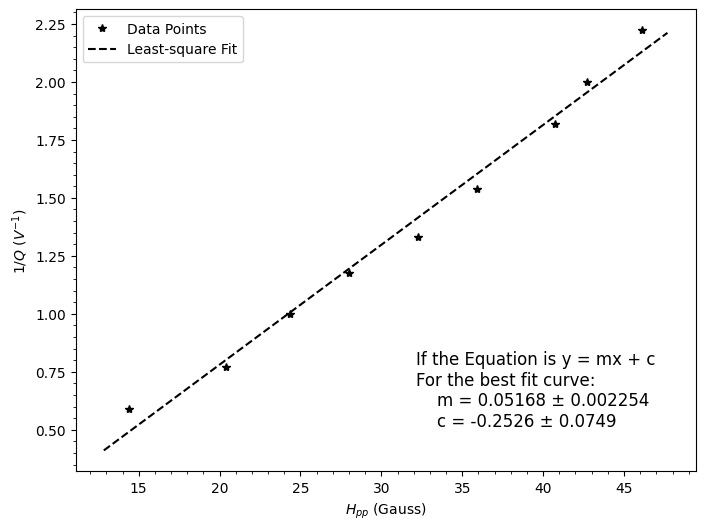
\includegraphics[width=1\columnwidth]{images/2.png}
    \caption{Plot of 1/Q vs. $H_{pp}$ at $\nu=14.01$ MHz}
    \label{g2}
\end{figure}

From Fig. \ref{g2}, slope $= 0.0517$. Putting $P=5$ V, we get $H_0=3.87$ Gauss and hence, $g=2.59$.

\begin{table}[H]
    \centering
        \caption{Table for measurement of $g$ at $\nu= 15.02$ MHz}
        \begin{tabular}{|c|c|c|c|c|} \hline
        Current (I) & 2Q & Q & Magnetic Field & $H_{pp}$ \\ 
        (mA) & (V) & (V) & H (mT) & (Gauss)\\ \hline
        99 & 3.4 & 1.70  & 0.51 & 14.42 \\
        127 & 2.6 & 1.30  & 0.72 & 20.36 \\
        154 & 2.0   & 1.00    & 0.86 & 24.32 \\
        184 & 1.7 & 0.85 & 0.99 & 28.00   \\
        209 & 1.5 & 0.75 & 1.14 & 32.24 \\
        233 & 1.3 & 0.65 & 1.27 & 35.92 \\
        258 & 1.1 & 0.55 & 1.44 & 40.73 \\
        282 & 1.0  & 0.50 & 1.51 & 42.71 \\
        307 & 0.9 & 0.45 & 1.63 & 46.10  \\ \hline
    \end{tabular}    
    \label{tab:3}
\end{table}

\begin{figure}[H]
    \centering
    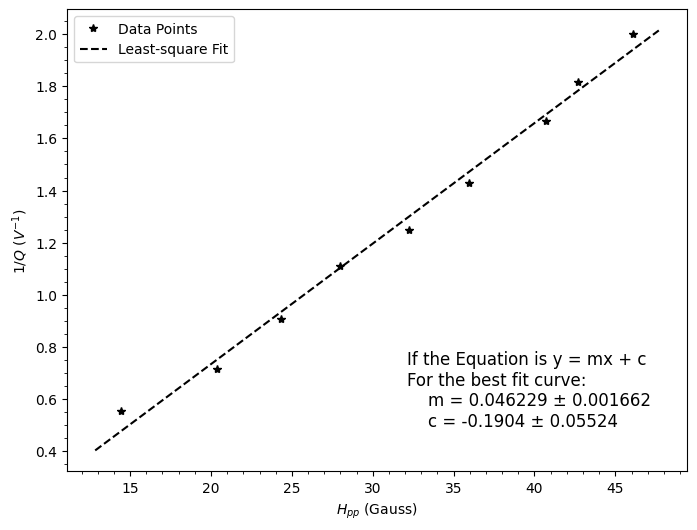
\includegraphics[width=1\columnwidth]{images/3.png}
    \caption{Plot of 1/Q vs. $H_{pp}$ at $\nu=15.02$ MHz}
    \label{g3}
\end{figure}

From Fig. \ref{g3}, slope $= 0.0462$. Putting $P=5$ V, we get $H_0=4.33$ Gauss and hence, $g=2.48$. And hence average value of $H_0=4.07$ Gauss and $g=2.46$.

\section{Error Analysis}

Error in $H_0$ will be given by,

\begin{align}
    \frac{\Delta H_0}{H_0} = \sqrt{\left(\frac{\Delta P}{P}\right)^2 + \left(\frac{\Delta \text{slope}}{\text{slope}}\right)^2}
\end{align}

And error in g will be given by,

\begin{align}
    \frac{\Delta g}{g} = \sqrt{\left(\frac{\Delta \nu}{\nu}\right)^2 + \left(\frac{\Delta H_0}{H_0}\right)^2}
\end{align}

Using $\Delta P = 0.2$ V and $\Delta \nu = 0.01$ MHz, plugging in the values:

\begin{itemize}
    \item For $\nu=13.03$ MHz,
    \begin{align*}
        \Delta H_{0_1} = 0.21 \text{ Gauss, } \Delta g_1 = 0.12
    \end{align*}
    \item For $\nu=14.01$ MHz,
    \begin{align*}
        \Delta H_{0_2} = 0.23 \text{ Gauss, } \Delta g_2 = 0.15
    \end{align*}
    \item For $\nu=15.02$ MHz,
    \begin{align*}
        \Delta H_{0_3} = 0.23 \text{ Gauss, } \Delta g_3 = 0.13
    \end{align*}
\end{itemize}

Avg. error in $H_0$,

\begin{align*}
    \Delta H_{0_\text{avg}} &= \frac{1}{3}\sqrt{(\Delta H_{0_1})^2 + (\Delta H_{0_2})^2 + (\Delta H_{0_2})^2}\\
    &= 0.13 \text{ Gauss}
\end{align*}

Avg. error in g,

\begin{align*}
    \Delta g_\text{avg} &= \frac{1}{3}\sqrt{(\Delta g_1)^2 + (\Delta g_2)^2 + (\Delta g_3)^2}= 0.08\\
\end{align*}

